\documentclass[11pt]{article}
\usepackage[a4paper,margin=1.05in]{geometry}
\usepackage{amsmath,amssymb,amsthm}
\usepackage{booktabs,array,graphicx,xcolor,enumitem}
\usepackage[colorlinks=true,linkcolor=blue!50!black,urlcolor=blue!50!black,citecolor=blue!50!black]{hyperref}
\usepackage{caption}
\captionsetup{font=small,labelfont=bf}
\newcommand{\NMAX}{13500}
\newcommand{\CountSix}{262}
\newcommand{\MeanD}{4.43}
\newcommand{\ReplayMax}{400000}
\newcommand{\TotalCases}{455173}
\newcommand{\DSixResidues}{11, 19}
\newcommand{\BallAThree}{874}
\newcommand{\BallBTwo}{123}
\newcommand{\BallBThree}{5599}
\newcommand{\MeetThree}{19}
\newcommand{\FirstSix}{163, 211, 283, 331, 523, 547, 571, 691}
\newcommand{\VerSha}{bd313fce5b368633}


\newtheorem{theorem}{Theorem}[section]
\newtheorem{lemma}[theorem]{Lemma}
\newtheorem{corollary}[theorem]{Corollary}
\theoremstyle{definition}
\newtheorem{definition}[theorem]{Definition}
\newtheorem{remark}[theorem]{Remark}
\newcommand{\N}{\mathbb{N}}
\newcommand{\dist}{\operatorname{d}}

\title{\textbf{Bounded Successor Distance in the Reversible\\ Square-Multiplication Graph}\\[4pt]
\large UNNS-U1-BND \,--\, version 1.0 (v001)}
\author{UNNS Research Collective}
\date{8 November 2026}

\begin{document}
\maketitle

\begin{abstract}
\noindent Let $G$ be the graph on the positive integers in which $kN$ is joined to $k(N+1)^2$ for all $k,N\ge 1$,
and let $\dist$ denote its graph distance. We prove that consecutive integers are always close:
$2\le \dist(n,n+1)\le 6$ for every $n\ge 1$, and the value $6$ is attained, so that
$\sup_{n}\dist(n,n+1)=6$. The upper bound is obtained from nine explicit path identities, one for each
residue class of $n$ modulo $4$, $8$ or $24$. In each class the path from $n$ to $n+1$ has a fixed number of steps
and its labels are linear polynomials in a class parameter; every step is certified by an integral, positive
cofactor, so legality holds for all members of the class at once. The lower bound is an exhaustive
meeting-in-the-middle computation at $n=163$, reproduced by two independent search programs. Consequently the
total distance along $1,2,\dots,k+1$ is at most $6k$.
\end{abstract}

\section{Introduction}\label{sec:intro}

\paragraph{Provenance.}
The graph $G$ is the undirected closure of the arithmetic transformation
$m\mapsto m(N+1)^2/N$ $(N\mid m)$ of the SELECT-II grammar of the UNNS Substrate: its forward edges are the legal
transitions and its inverse edges are their inverses. Forward-only properties of this transformation (its exact
one-step image, orbit criterion and label-realizability criterion) are the subject of research note U0-001 \cite{u0}.
The connectivity of $G$ is established in the preceding note \cite{u1}, which is kept as a provisional baseline.
The present release, UNNS-U1-BND, is independent of both: it leaves them, and the frozen reference collection
\cite{gig,repo}, unchanged. Its question is quantitative. Given that $G$ is connected, how far apart can
\emph{consecutive} integers be?

\paragraph{Result.}
\begin{theorem}[Bounded successor distance]\label{thm:main}
For every integer $n\ge 1$, $\;2\le \dist(n,n+1)\le 6$. Moreover $\dist(163,164)=6$. Hence
\[
C_\ast:=\sup_{n\ge 1}\dist(n,n+1)=6 .
\]
\end{theorem}

\paragraph{Mechanism.}
The identities share one idea: a forward step produces a number carrying a large square factor built from $n$ or
$n+1$, and the surplus is then traded for the target by inverse steps whose labels are linear in a class parameter.
Which linear forms are integral depends on $n$ modulo $8$ and, in the hardest classes, modulo $3$; this is why the
constant becomes $6$ only after splitting modulo $24$ (Section~\ref{sec:upper}).

\paragraph{Organization.}
Section~\ref{sec:prelim} fixes notation. Section~\ref{sec:upper} proves the upper bound; Section~\ref{sec:lower}
the sharpness. Section~\ref{sec:data} reports the exact distances computed. Section~\ref{sec:status} separates what is proved
from what is only computed. Section~\ref{sec:open} lists open questions. Appendix~\ref{app:cert} contains the complete
step-by-step certificates.

\section{Preliminaries}\label{sec:prelim}

\begin{definition}
$G$ has vertex set $\N_{>0}$ and an edge $\{kN,\,k(N+1)^2\}$ for each pair $k,N\ge 1$. A \emph{forward step with
label $N$} replaces $x=kN$ by $k(N+1)^2$; an \emph{inverse step with label $N$} replaces $x=k(N+1)^2$ by $kN$.
The number $k$ is the \emph{cofactor} of the step. $\dist$ is the shortest-path distance.
\end{definition}

A forward step with label $N$ is legal exactly when $N\mid x$; an inverse step with label $N$ exactly when
$(N+1)^2\mid x$. Each vertex has finitely many neighbours (forward labels are divisors of $x$, inverse labels satisfy
$(N+1)^2\mid x$), so $G$ is locally finite and balls of finite radius are finite, computable sets.

\begin{lemma}[Edge criterion]\label{lem:edge}
For $x<y$, $x\sim y$ if and only if $y=x(N+1)^2/N$ for some integer $N\ge1$ with $N\mid x$, and then $N$ is a positive
root of $N^2+(2-y/x)N+1=0$.
\end{lemma}
\begin{proof}
Immediate from the definition; $y/x=(N+1)^2/N$ rearranges to the stated quadratic.
\end{proof}

\begin{lemma}[Consecutive integers are never adjacent]\label{lem:nonadj}
$\dist(n,n+1)\ge 2$ for all $n\ge1$.
\end{lemma}
\begin{proof}
An edge multiplies by $(N+1)^2/N=N+2+1/N\ge 4$, whereas $(n+1)/n\le 2$.
\end{proof}

\section{The upper bound: nine path identities}\label{sec:upper}

Table~\ref{tab:ident} lists the identities. In it $+N$ denotes a forward step and $-N$ an inverse step with label
$N$; $t$ is a nonnegative integer parameter with the stated lower limit.

\begin{table}[h]\centering\small
\begin{tabular}{@{}clcl@{}}
\toprule
class & $n$ & steps & labels (forward $+N$, inverse $-N$) \\ \midrule
A & $n=4t+1$\,($t\ge 1$) & 4 & $+(4 t + 1)$,\ $-2 t$,\ $+t$,\ $-(2 t + 1)$ \\
B & $n=8t$\,($t\ge 1$) & 5 & $+2$,\ $+2$,\ $-8$,\ $+4 t$,\ $-(8 t + 1)$ \\
C & $n=8t+2$\,($t\ge 0$) & 5 & $+2$,\ $+(4 t + 1)$,\ $+2$,\ $-8$,\ $-(8 t + 3)$ \\
D & $n=8t+4$\,($t\ge 0$) & 5 & $+2$,\ $+2$,\ $-8$,\ $+(2 \left(2 t + 1\right))$,\ $-(8 t + 5)$ \\
E & $n=8t+6$\,($t\ge 0$) & 5 & $+2$,\ $+(4 t + 3)$,\ $+2$,\ $-8$,\ $-(8 t + 7)$ \\
F & $n=24t+3$\,($t\ge 1$) & 4 & $+(8 t + 1)$,\ $-4 t$,\ $+3 t$,\ $-(6 t + 1)$ \\
G & $n=8t+7$\,($t\ge 0$) & 6 & $+(8 t + 7)$,\ $+(t + 1)$,\ $+(t + 1)$,\ $-(2 t + 3)$,\ $-(2 t + 3)$,\ $-(2 \left(t + 1\right))$ \\
H & $n=24t+11$\,($t\ge 0$) & 6 & $+(24 t + 11)$,\ $+24$,\ $-(2 \left(25 t + 12\right))$,\ $+(25 t + 12)$,\ $-(25 \left(2 t + 1\right))$,\ $-4$ \\
I & $n=24t+19$\,($t\ge 0$) & 6 & $+1$,\ $+(24 t + 19)$,\ $-3$,\ $-(3 \left(4 t + 3\right))$,\ $+(4 t + 3)$,\ $-(6 t + 5)$ \\
\bottomrule
\end{tabular}

\caption{The nine path identities carrying $n$ to $n+1$. Every integer $n\ge 2$ except $n=3$ lies in exactly one class
(Lemma~\ref{lem:cover}).}\label{tab:ident}
\end{table}

\begin{lemma}[Certified identities give paths]\label{lem:cert}
Fix a class $n=Mt+r$ with limit $t_0$ and a list of steps $(\varepsilon_i,N_i(t))_{i=1}^{L}$. Suppose polynomials
$s_0(t)=Mt+r,\ s_1(t),\dots,s_L(t)=Mt+r+1$ and $k_1(t),\dots,k_L(t)$ satisfy, for each $i$,
\[
\begin{aligned}
&\text{forward: } s_{i-1}=k_iN_i,\ \ s_i=k_i(N_i+1)^2;\\
&\text{inverse: } s_{i-1}=k_i(N_i+1)^2,\ \ s_i=k_iN_i,
\end{aligned}
\]
and that all $N_i(t)$ and $k_i(t)$ are integers $\ge1$ for every integer $t\ge t_0$. Then for every such $t$ the
sequence $s_0(t),\dots,s_L(t)$ is a walk in $G$ from $n$ to $n+1$ of length $L$.
\end{lemma}
\begin{proof}
Each consecutive pair is, by the displayed relations, an edge $\{kN,k(N+1)^2\}$ with integers $k,N\ge1$.
\end{proof}

\paragraph{A worked identity (class A).}
Let $n=4t+1$ with $t\ge1$. The walk is
\[
4t+1\ \xrightarrow{+\,(4t+1)}\ 4(2t+1)^2\ \xrightarrow{-\,2t}\ 8t\ \xrightarrow{+\,t}\ 8(t+1)^2\ \xrightarrow{-\,(2t+1)}\ 2(2t+1)=n+1 .
\]
Indeed: (1) $4t+1=kN$ with $k=1$, $N=4t+1$, giving $(4t+2)^2=4(2t+1)^2$. (2) $4(2t+1)^2=k(N+1)^2$ with $N=2t$, $k=4$, giving
$kN=8t$. (3) $8t=kN$ with $N=t$, $k=8$, giving $8(t+1)^2$. (4) $8(t+1)^2=k(N+1)^2$ with $N=2t+1$ and $k=2$ (because
$(N+1)^2=4(t+1)^2$), giving $kN=2(2t+1)=n+1$. All labels and cofactors are positive integers for $t\ge1$.

\paragraph{A second worked identity (class G).}
Let $n=8t+7$, so $n+1=8(t+1)$. The walk is
\[
\begin{aligned}
8t+7 &\xrightarrow{+(8t+7)} 64(t+1)^2 \xrightarrow{+(t+1)} 64(t+1)(t+2)^2 \xrightarrow{+(t+1)} 64(t+2)^4\\
&\xrightarrow{-(2t+3)} 16(t+2)^2(2t+3)\xrightarrow{-(2t+3)} 4(2t+3)^2 \xrightarrow{-2(t+1)} 8(t+1)=n+1 .
\end{aligned}
\]
The steps have labels and cofactors $(N,k)$ equal to: $(8t+7,\,1)$; $(t+1,\,64(t+1))$; $(t+1,\,64(t+2)^2)$;
$(2t+3,\,16(t+2)^2)$ [using $(N+1)^2=4(t+2)^2$]; $(2t+3,\,4(2t+3))$ [same square]; and $(2t+2,\,4)$ [using $(N+1)^2=(2t+3)^2$].
In each forward step the state equals $kN$ and the next state $k(N+1)^2$; in each inverse step the state equals $k(N+1)^2$ and the
next state $kN$. All of these are positive integers for every $t\ge0$.

\begin{lemma}[Coverage]\label{lem:cover}
Every integer $n\ge1$ is either $1$ or $3$, or lies in exactly one class: $n\equiv1\pmod 4$ is class A;
$n\equiv 0,2,4,6\pmod 8$ are classes B, C, D, E; $n\equiv 7\pmod 8$ is class G; and $n\equiv 3\pmod 8$ is
class F, H or I according as $n\equiv 3,11,19\pmod{24}$. For $n=1$ and $n=3$ the explicit walks
$1,4,18,81,8,2$ and $3,16,4$ have lengths $5$ and $2$.
\end{lemma}
\begin{proof}
The residues listed partition the integers; classes A, B and F require $t\ge1$, which excludes only $n=1$ (class A at $t=0$)
and $n=3$ (class F at $t=0$). The walk $1,4,18,81,8,2$ uses the edges $\{1\cdot1,\,1\cdot2^2\}$, $\{2\cdot2,\,2\cdot3^2\}$, $\{9\cdot2,\,9\cdot3^2\}$, $\{1\cdot8,\,1\cdot9^2\}$
(traversed backwards) and $\{2\cdot1,\,2\cdot2^2\}$ (backwards); the walk $3,16,4$ uses $\{1\cdot3,\,1\cdot4^2\}$ and $\{4\cdot1,\,4\cdot2^2\}$ (backwards).
\end{proof}

\begin{figure}[h]\centering
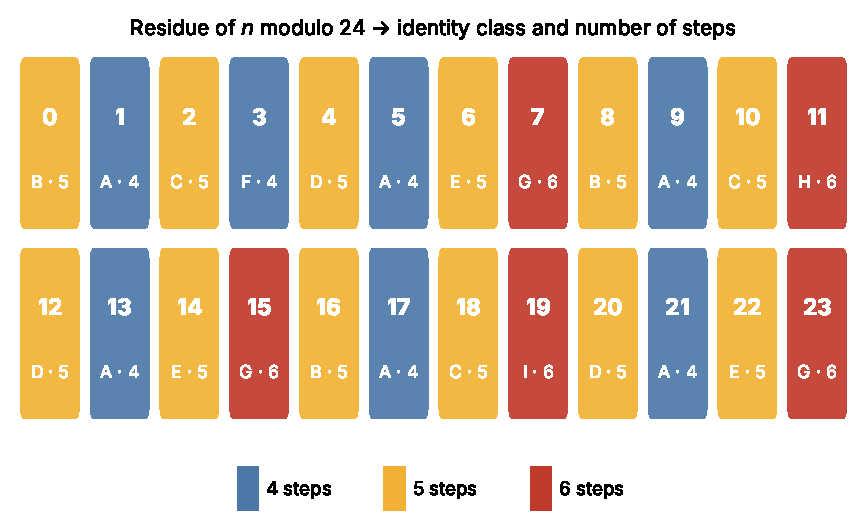
\includegraphics[width=.86\textwidth]{figures/fig1_residue_cover.pdf}
\caption{Residue classes modulo $24$ and the identity (letter) assigned to each, with its number of steps.
Only residues $7,11,15,19,23$ require six steps; classes F and A need four.}\label{fig:cover}
\end{figure}

\begin{proof}[Proof of the upper bound in Theorem~\ref{thm:main}]
By Lemma~\ref{lem:cover} it suffices to certify the nine identities. Appendix~\ref{app:cert} gives, for each identity and
each step, the label, the cofactor $k_i(t)$, and the states $s_{i-1}(t)$, $s_i(t)$ as explicit polynomials; each row is
checked by one multiplication. All labels and cofactors are integer-valued polynomials with nonnegative
coefficients and value $\ge1$ at $t=t_0$, so they are integers $\ge1$ for all $t\ge t_0$. Lemma~\ref{lem:cert} then gives walks of length at most $6$.
Together with Lemma~\ref{lem:nonadj} this proves $2\le\dist(n,n+1)\le 6$.
\end{proof}

\begin{remark}[Refinement matters]
Using only residues modulo $8$, the search found for the class $n\equiv3\pmod 8$ a uniform identity of length $7$ and none
shorter within its vocabulary of linear and quadratic label forms. Splitting it modulo $24$ yields identities F, H, I of lengths $4$, $6$, $6$. The constant
$C_\ast=6$ therefore depends on distinguishing $n$ modulo $3$ in this class.
\end{remark}

\section{Sharpness: the lower bound at $n=163$}\label{sec:lower}

\begin{lemma}[Meeting in the middle]\label{lem:mitm}
If $\dist(a,b)=t$ then $B_{\lceil t/2\rceil}(a)\cap B_{\lfloor t/2\rfloor}(b)\neq\emptyset$, where $B_r(x)$ is the set of vertices
within distance $r$ of $x$. In particular, $B_3(a)\cap B_2(b)=\emptyset$ implies $\dist(a,b)\ge6$.
\end{lemma}
\begin{proof}
The vertex at position $\lceil t/2\rceil$ along a shortest path lies in both balls. If $t\le5$ then
$\lceil t/2\rceil\le3$ and $\lfloor t/2\rfloor\le2$, and balls grow with the radius.
\end{proof}

\begin{theorem}[Lower bound]\label{thm:lower}
$\dist(163,164)=6$.
\end{theorem}
\begin{proof}[Proof (exhaustive computation)]
Balls are finite and computable by local finiteness. Enumerating them without any size cap gives
$|B_3(163)|=\BallAThree$ and $|B_2(164)|=\BallBTwo$, and $B_3(163)\cap B_2(164)=\emptyset$; by Lemma~\ref{lem:mitm},
$\dist(163,164)\ge6$. Enumerating $B_3(164)$ ($\BallBThree$ vertices) gives $\MeetThree$ common vertices with $B_3(163)$,
so a walk of length $6$ exists (and identity I produces one explicitly: Figure~\ref{fig:paths}). The computation was
performed by two independent programs (one factoring neighbours with Pollard's method, one using only trial division);
their ball sizes and intersections agree (check V8).
\end{proof}

The same computation gives $\dist(211,212)=\dist(283,284)=6$; the first values with $\dist(n,n+1)=6$ are
$\FirstSix$.

\begin{figure}[h]\centering
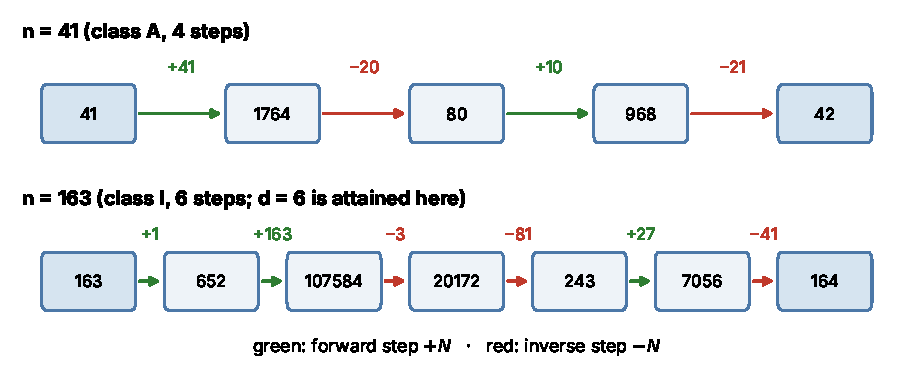
\includegraphics[width=.95\textwidth]{figures/fig3_example_paths.pdf}
\caption{Two concrete walks produced by the identities: $n=41$ by identity A (four steps) and $n=163$ by identity I
(six steps, optimal).}\label{fig:paths}
\end{figure}

\begin{corollary}[Linear cumulative cost]\label{cor:cum}
$\sum_{n=1}^{k}\dist(n,n+1)\le 6k$ for every $k\ge1$; a walk through $1,2,\dots,k+1$ in order exists with at most $6k$ steps.
\end{corollary}

\section{Exact distances in the computed range}\label{sec:data}

Using the exact search for every $n\le\NMAX$ we obtain the distribution of Table~\ref{tab:dist}; the mean is $\MeanD$.
The value $6$ occurs $\CountSix$ times in this range, and only at residues $\DSixResidues$ modulo $24$. This is consistent with
Section~\ref{sec:upper}: a value $6$ can only occur where the assigned identity has length $6$.

\begin{table}[h]\centering\small
\begin{tabular}{@{}lrrrrr@{}}
\toprule
$d(n,n+1)$ & $2$ & $3$ & $4$ & $5$ & $6$ \\
count & 2 & 23 & 7875 & 5338 & 262 \\
\bottomrule
\end{tabular}

\caption{Exact $\dist(n,n+1)$ for $1\le n\le\NMAX$ (data file \texttt{successor\_distance\_table.csv}).}\label{tab:dist}
\end{table}

\begin{figure}[h]\centering
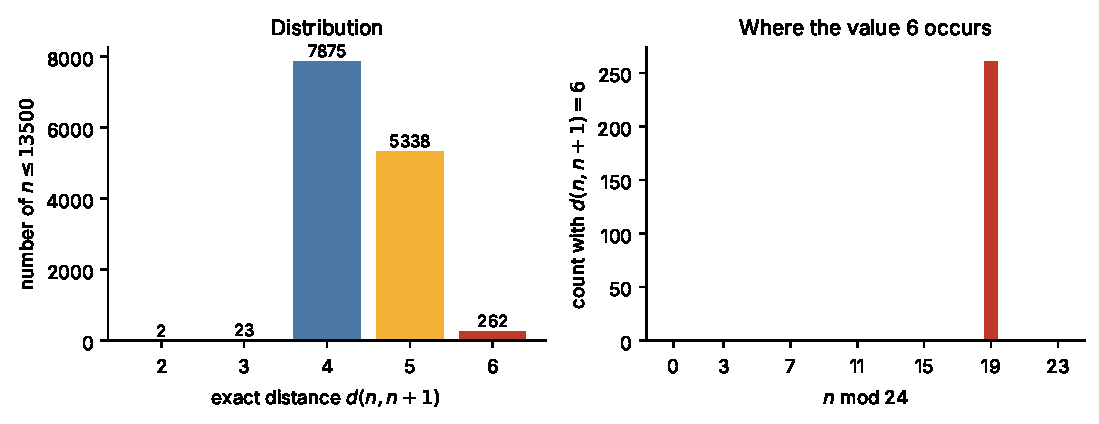
\includegraphics[width=.95\textwidth]{figures/fig2_distance_distribution.pdf}
\caption{Left: distribution of exact distances. Right: residues modulo $24$ at which $\dist(n,n+1)=6$ occurs
within the computed range.}\label{fig:dist}
\end{figure}

\begin{remark}
Computation alone cannot show that $\dist(n,n+1)=6$ occurs infinitely often; it is observed $\CountSix$ times below $\NMAX$.
The theorem only asserts that the supremum equals $6$.
\end{remark}

\section{Status of the results}\label{sec:status}

\begin{center}\small
\begin{tabular}{@{}p{0.47\textwidth}p{0.43\textwidth}@{}}\toprule
Statement & Status\\ \midrule
Upper bound $\dist(n,n+1)\le6$ & Proved: Lemmas~\ref{lem:cert},~\ref{lem:cover} and the certificates; computer-algebra verified; classes A and G checked by hand in the text\\
Lower bound $\dist(n,n+1)\ge2$ & Proved (Lemma~\ref{lem:nonadj})\\
Sharpness $\dist(163,164)=6$ & Exhaustive computation, two independent programs; not a hand proof\\
Occurrence of the value $6$ for infinitely many $n$ & Not established\\
Connectivity of $G$ & Context only (preceding note \cite{u1}); constructive paths re-checked for $n\le1500$ (V5)\\
Proof-assistant certification & Not performed\\
Originality relative to prior literature & Not reviewed\\ \bottomrule
\end{tabular}
\end{center}

Table~\ref{tab:checks} lists the finite computations. The symbolic check V2 is an exact computer-algebra statement
(\texttt{sympy} \cite{sympy}); the others are finite computations over the stated ranges and support, but do not replace, the proofs above.
\begin{table}[h]\centering\small
\begin{tabular}{@{}llrl@{}}
\toprule
check & what it tests & cases & result \\ \midrule
V1 & closed-form edge test equals the definition & 40000 & pass \\
V2 & exact symbolic certificates for the nine identities & 9 & pass \\
V3 & coverage of all residues modulo 24; special paths for $n=1,3$ & 97 & pass \\
V4 & plain-integer replay of every identity with edge test & 400000 & pass \\
V5 & constructive connectivity paths (context) & 1500 & pass \\
V6 & exact distance table, consistency with identity lengths & 13500 & pass \\
V7 & independent engine reproduces distances & 62 & pass \\
V8 & lower-bound certificate at $n=163$, two engines & 3 & pass \\
V9 & trivial lower bound $d(n,n+1)\ge 2$ & 2 & pass \\
\bottomrule
\end{tabular}

\caption{Verification checks ($\TotalCases$ cases in total, deterministic exact arithmetic, report \texttt{u1\_bnd\_verification\_report.json}).}\label{tab:checks}
\end{table}

\section{Consequences and observations}\label{sec:cons}

\paragraph{Waypoint cost.}
By Corollary~\ref{cor:cum}, the sequence $1,2,3,\dots$ has bounded \emph{amortized} waypoint cost in $G$: at most six
legal transitions per successor, whatever the magnitude of $n$; in the computed range the mean is $\MeanD$.

\paragraph{What this does and does not say.}
The identities are uniform programs of fixed length with $n$ entering only through a class parameter; to apply one it
suffices to know which of finitely many residue classes contains $n$. This is a statement about the geometry of $G$.
It is \emph{not} a selector: it does not show that a rule computing each next label from the current state alone,
without being told the target, reproduces the integers. That question is separate.

\section{Open questions}\label{sec:open}
\begin{enumerate}[leftmargin=*]
\item Does $\dist(n,n+1)=6$ occur for infinitely many $n$? Is there a density statement in classes H and I?
\item Which residue classes modulo larger moduli admit uniform identities shorter than those above, and which are exact?
\item For which rational functions $f$ is $\sup_n\dist(n,f(n))$ finite (for example $f(n)=2n,\ n+2,\ n^2$)? The search
method used here (in \texttt{code/search}) finds candidate identities for such pairs.
\item The growth of $\dist(1,n)$: the coarse bound known from the preceding note is linear; the true growth rate is unknown.
\item Can a fixed state-computable rule select the labels, so that the successor transition is generated rather than
supplied?
\end{enumerate}

\appendix
\section{Complete step certificates}\label{app:cert}
Each row records one step: type, label $N$, cofactor $k$, and the states before and after. A forward row satisfies
(before)$=kN$ and (after)$=k(N+1)^2$; an inverse row satisfies (before)$=k(N+1)^2$ and (after)$=kN$.
These tables are generated from the symbolic certificates (check V2).
\paragraph{Identity A: $n=4t+1$, $t\ge 1$ (4 steps).}
\begin{center}\footnotesize
\begin{tabular}{@{}clcccc@{}}\toprule
step & type & $N$ & cofactor $k$ & state before & state after \\ \midrule
1 & forward & $4 t + 1$ & $1$ & $4 t + 1$ & $4 \left(2 t + 1\right)^{2}$ \\
2 & inverse & $2 t$ & $4$ & $4 \left(2 t + 1\right)^{2}$ & $8 t$ \\
3 & forward & $t$ & $8$ & $8 t$ & $8 \left(t + 1\right)^{2}$ \\
4 & inverse & $2 t + 1$ & $2$ & $8 \left(t + 1\right)^{2}$ & $2 \left(2 t + 1\right)$ \\
\bottomrule\end{tabular}\end{center}
\paragraph{Identity B: $n=8t$, $t\ge 1$ (5 steps).}
\begin{center}\footnotesize
\begin{tabular}{@{}clcccc@{}}\toprule
step & type & $N$ & cofactor $k$ & state before & state after \\ \midrule
1 & forward & $2$ & $4 t$ & $8 t$ & $36 t$ \\
2 & forward & $2$ & $18 t$ & $36 t$ & $162 t$ \\
3 & inverse & $8$ & $2 t$ & $162 t$ & $16 t$ \\
4 & forward & $4 t$ & $4$ & $16 t$ & $4 \left(4 t + 1\right)^{2}$ \\
5 & inverse & $8 t + 1$ & $1$ & $4 \left(4 t + 1\right)^{2}$ & $8 t + 1$ \\
\bottomrule\end{tabular}\end{center}
\paragraph{Identity C: $n=8t+2$, $t\ge 0$ (5 steps).}
\begin{center}\footnotesize
\begin{tabular}{@{}clcccc@{}}\toprule
step & type & $N$ & cofactor $k$ & state before & state after \\ \midrule
1 & forward & $2$ & $4 t + 1$ & $2 \left(4 t + 1\right)$ & $9 \left(4 t + 1\right)$ \\
2 & forward & $4 t + 1$ & $9$ & $9 \left(4 t + 1\right)$ & $36 \left(2 t + 1\right)^{2}$ \\
3 & forward & $2$ & $18 \left(2 t + 1\right)^{2}$ & $36 \left(2 t + 1\right)^{2}$ & $162 \left(2 t + 1\right)^{2}$ \\
4 & inverse & $8$ & $2 \left(2 t + 1\right)^{2}$ & $162 \left(2 t + 1\right)^{2}$ & $16 \left(2 t + 1\right)^{2}$ \\
5 & inverse & $8 t + 3$ & $1$ & $16 \left(2 t + 1\right)^{2}$ & $8 t + 3$ \\
\bottomrule\end{tabular}\end{center}
\paragraph{Identity D: $n=8t+4$, $t\ge 0$ (5 steps).}
\begin{center}\footnotesize
\begin{tabular}{@{}clcccc@{}}\toprule
step & type & $N$ & cofactor $k$ & state before & state after \\ \midrule
1 & forward & $2$ & $2 \left(2 t + 1\right)$ & $4 \left(2 t + 1\right)$ & $18 \left(2 t + 1\right)$ \\
2 & forward & $2$ & $9 \left(2 t + 1\right)$ & $18 \left(2 t + 1\right)$ & $81 \left(2 t + 1\right)$ \\
3 & inverse & $8$ & $2 t + 1$ & $81 \left(2 t + 1\right)$ & $8 \left(2 t + 1\right)$ \\
4 & forward & $2 \left(2 t + 1\right)$ & $4$ & $8 \left(2 t + 1\right)$ & $4 \left(4 t + 3\right)^{2}$ \\
5 & inverse & $8 t + 5$ & $1$ & $4 \left(4 t + 3\right)^{2}$ & $8 t + 5$ \\
\bottomrule\end{tabular}\end{center}
\paragraph{Identity E: $n=8t+6$, $t\ge 0$ (5 steps).}
\begin{center}\footnotesize
\begin{tabular}{@{}clcccc@{}}\toprule
step & type & $N$ & cofactor $k$ & state before & state after \\ \midrule
1 & forward & $2$ & $4 t + 3$ & $2 \left(4 t + 3\right)$ & $9 \left(4 t + 3\right)$ \\
2 & forward & $4 t + 3$ & $9$ & $9 \left(4 t + 3\right)$ & $144 \left(t + 1\right)^{2}$ \\
3 & forward & $2$ & $72 \left(t + 1\right)^{2}$ & $144 \left(t + 1\right)^{2}$ & $648 \left(t + 1\right)^{2}$ \\
4 & inverse & $8$ & $8 \left(t + 1\right)^{2}$ & $648 \left(t + 1\right)^{2}$ & $64 \left(t + 1\right)^{2}$ \\
5 & inverse & $8 t + 7$ & $1$ & $64 \left(t + 1\right)^{2}$ & $8 t + 7$ \\
\bottomrule\end{tabular}\end{center}
\paragraph{Identity F: $n=24t+3$, $t\ge 1$ (4 steps).}
\begin{center}\footnotesize
\begin{tabular}{@{}clcccc@{}}\toprule
step & type & $N$ & cofactor $k$ & state before & state after \\ \midrule
1 & forward & $8 t + 1$ & $3$ & $3 \left(8 t + 1\right)$ & $12 \left(4 t + 1\right)^{2}$ \\
2 & inverse & $4 t$ & $12$ & $12 \left(4 t + 1\right)^{2}$ & $48 t$ \\
3 & forward & $3 t$ & $16$ & $48 t$ & $16 \left(3 t + 1\right)^{2}$ \\
4 & inverse & $6 t + 1$ & $4$ & $16 \left(3 t + 1\right)^{2}$ & $4 \left(6 t + 1\right)$ \\
\bottomrule\end{tabular}\end{center}
\paragraph{Identity G: $n=8t+7$, $t\ge 0$ (6 steps).}
\begin{center}\footnotesize
\begin{tabular}{@{}clcccc@{}}\toprule
step & type & $N$ & cofactor $k$ & state before & state after \\ \midrule
1 & forward & $8 t + 7$ & $1$ & $8 t + 7$ & $64 \left(t + 1\right)^{2}$ \\
2 & forward & $t + 1$ & $64 \left(t + 1\right)$ & $64 \left(t + 1\right)^{2}$ & $64 \left(t + 1\right) \left(t + 2\right)^{2}$ \\
3 & forward & $t + 1$ & $64 \left(t + 2\right)^{2}$ & $64 \left(t + 1\right) \left(t + 2\right)^{2}$ & $64 \left(t + 2\right)^{4}$ \\
4 & inverse & $2 t + 3$ & $16 \left(t + 2\right)^{2}$ & $64 \left(t + 2\right)^{4}$ & $16 \left(t + 2\right)^{2} \left(2 t + 3\right)$ \\
5 & inverse & $2 t + 3$ & $4 \left(2 t + 3\right)$ & $16 \left(t + 2\right)^{2} \left(2 t + 3\right)$ & $4 \left(2 t + 3\right)^{2}$ \\
6 & inverse & $2 \left(t + 1\right)$ & $4$ & $4 \left(2 t + 3\right)^{2}$ & $8 \left(t + 1\right)$ \\
\bottomrule\end{tabular}\end{center}
\paragraph{Identity H: $n=24t+11$, $t\ge 0$ (6 steps).}
\begin{center}\footnotesize
\begin{tabular}{@{}clcccc@{}}\toprule
step & type & $N$ & cofactor $k$ & state before & state after \\ \midrule
1 & forward & $24 t + 11$ & $1$ & $24 t + 11$ & $144 \left(2 t + 1\right)^{2}$ \\
2 & forward & $24$ & $6 \left(2 t + 1\right)^{2}$ & $144 \left(2 t + 1\right)^{2}$ & $3750 \left(2 t + 1\right)^{2}$ \\
3 & inverse & $2 \left(25 t + 12\right)$ & $6$ & $3750 \left(2 t + 1\right)^{2}$ & $12 \left(25 t + 12\right)$ \\
4 & forward & $25 t + 12$ & $12$ & $12 \left(25 t + 12\right)$ & $12 \left(25 t + 13\right)^{2}$ \\
5 & inverse & $25 \left(2 t + 1\right)$ & $3$ & $12 \left(25 t + 13\right)^{2}$ & $75 \left(2 t + 1\right)$ \\
6 & inverse & $4$ & $3 \left(2 t + 1\right)$ & $75 \left(2 t + 1\right)$ & $12 \left(2 t + 1\right)$ \\
\bottomrule\end{tabular}\end{center}
\paragraph{Identity I: $n=24t+19$, $t\ge 0$ (6 steps).}
\begin{center}\footnotesize
\begin{tabular}{@{}clcccc@{}}\toprule
step & type & $N$ & cofactor $k$ & state before & state after \\ \midrule
1 & forward & $1$ & $24 t + 19$ & $24 t + 19$ & $4 \left(24 t + 19\right)$ \\
2 & forward & $24 t + 19$ & $4$ & $4 \left(24 t + 19\right)$ & $64 \left(6 t + 5\right)^{2}$ \\
3 & inverse & $3$ & $4 \left(6 t + 5\right)^{2}$ & $64 \left(6 t + 5\right)^{2}$ & $12 \left(6 t + 5\right)^{2}$ \\
4 & inverse & $3 \left(4 t + 3\right)$ & $3$ & $12 \left(6 t + 5\right)^{2}$ & $9 \left(4 t + 3\right)$ \\
5 & forward & $4 t + 3$ & $9$ & $9 \left(4 t + 3\right)$ & $144 \left(t + 1\right)^{2}$ \\
6 & inverse & $6 t + 5$ & $4$ & $144 \left(t + 1\right)^{2}$ & $4 \left(6 t + 5\right)$ \\
\bottomrule\end{tabular}\end{center}


\section{Reproducibility}
The package contains the verifier (\texttt{code/verify\_u1\_bnd.py}, SHA-256 prefix \VerSha{}), the library with the engines
and identities, the search tool used to discover the identities, the exact-distance table, the machine-readable
identity record and the verification report. Run \texttt{python3 verify\_u1\_bnd.py} inside \texttt{code/} (requires Python 3 and
\texttt{sympy}); the report is deterministic.

\begin{thebibliography}{9}\small
\bibitem{u0} UNNS Research Collective, \emph{UNNS-U0: Arithmetic reachability and orbit admissibility}, research note U0-001, 8 November 2026
(local release; not part of the frozen repository).
\bibitem{u1} UNNS Research Collective, \emph{UNNS-U1: Reversible arithmetic connectivity}, research note, 8 November 2026
(provisional baseline; local release).
\bibitem{gig} UNNS Research Collective, \emph{UNNS Generative Information Geometry collection}, frozen release, repository \texttt{ukbbi/UNNS}, commit
\texttt{a115e4bc6b8ee734e6146b3b17a6b121e65d31c3}:
\url{https://github.com/ukbbi/UNNS/tree/a115e4bc6b8ee734e6146b3b17a6b121e65d31c3/projects/UNNS_Generative_Information_Geometry}.
\bibitem{repo} UNNS project repository, pinned at the same commit:
\url{https://github.com/ukbbi/UNNS/tree/a115e4bc6b8ee734e6146b3b17a6b121e65d31c3}.
\bibitem{sympy} A. Meurer et al., SymPy: symbolic computing in Python, \emph{PeerJ Computer Science} \textbf{3} (2017), e103,
\url{https://doi.org/10.7717/peerj-cs.103}.
\end{thebibliography}
\end{document}
